\documentclass{report}

%%%%%%%%%%%%%%%%%%%%%%%%%% Practice info %%%%%%%%%%%%%%%%%%%%%%%%%%
\Subject {Системи штучного інтелекту}
\LabTitle{MNIST: розпізнавання рукописних цифр}
\LabReport{Практична робота \#4}

\Done{Виконав:}  % Поставте правильне закінчення

%%%%%%%%%%%%%%%%%%%%%%%%%% Your personal data %%%%%%%%%%%%%%%%%%%%%%%%%%
\Surname{Коваль}
\Name{Ростислав}
\Group {ІО-11мн}
\YearOfStudying {1}

%%%%%%%%%%%%%%%%%%%%%%%%%% starting the document %%%%%%%%%%%%%%%%%%%%%%%%
\startDocument


\section{MNIST: розпізнавання рукописних цифр}

\subsection{Набір даних}
Для виконання цього завдання було використано набір даних MNIST in CSV~\cite{kaggleMNIST}.

Набір даних: для навчання було використано 58471 рядків з CSV файлу даних, для валідації 1000 рядків. Остаточне тестування проходило на валідаційному наборі даних теж з 1000 значень.
Роздільна здатність зображень - (28, 28, 1).
Дані не ділив на 255, залишив їх в діапазоні від 0 до 255. Була виконана попередня обробка даних: змінив розмір файлів, перетворив їх з (786, ) - на розмір (28, 28, 1). Нормалізація і збільшення даних не використовувалося.
Приклади зображень:


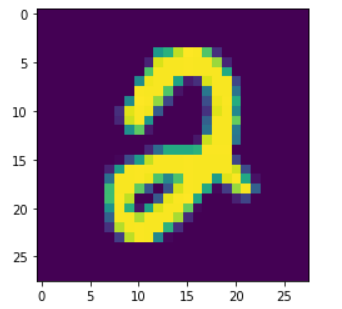
\includegraphics{images/2.png}
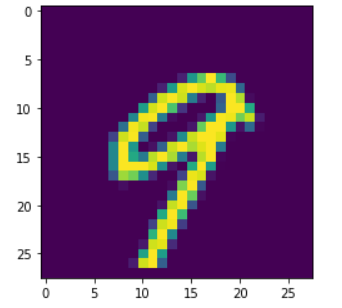
\includegraphics{images/9.png}
\subsection{Структура моделі}
Моя модель має 3 шари, перший для перетворення даних в одновимірний масив, 2 наступні - повнозв'язні шари, в першому повнозв'язному 128 нейронів та функція активації relu та в останньому 10 нейронів та активація softmax. 10 нейронів відображають кількість наших класів. Для функції витрат була використана SparseCategoricalCrossentropy так як лейбли не були у форматі one-hot encoding. Оптимізатор RMSprop з дефолтними параметрами. Модель була натренована протягом 100 епох з batch-size = 64.

\begin{lstlisting}[language=Python, style=mypython, caption={Модель}]
# Creating model architecture, setting parameters: loss function, metrics and optimizer. 
# Start training for 100 epochs.
mdl = tf.keras.Sequential([tf.keras.layers.Flatten(input_shape=(pix, pix, 1)), tf.keras.layers.Dense(128, activation='relu'),tf.keras.layers.Dense(10, activation="softmax")])
mdl.compile(optimizer=tf.keras.optimizers.RMSprop(), loss=tf.keras.losses.SparseCategoricalCrossentropy(), metrics=['accuracy'])
mdl.fit(x_train, y_train, epochs=100, batch_size=64)
\end{lstlisting}

\subsection{Результати експериментів}
У даній роботі я не змінював гіперпараметри, використовувалася параметри за замовчуванням. Наприклад, learning rate = 0.001.
Основна метрика у моїй роботі - це точність (accuracy).
Вона визначається як відношення кількості зображень, які правильно визначила модель до всієї кількості фотографій.
\subsection{Допомога}
Не отримував допомоги від інших людей, використовував наступні матеріали:
~\cite{kaggle1, kaggle2, kaggle3, kaggle4, tensorflow}.

\subsection{Висновки}
Дана архітектура була обрана, бо це найпростіший варіант для вирішення задачі класифікацї на датасеті MNIST. Я не змінював гіперпараметри, вони використовували значення за замовчуванням.
Також я зміг отримати більшу точність при збільшенні кількості епох з 50 до 100, якщо обирати кількість більшу за 100 - точність залишається майже тою ж самою. В результаті точність визначення цифр на kaggle становить 0.96936.
\newpage
%%%%%%%%%%%%%%%%%% Література %%%%%%%%%%%%%%%%%%%%%%%%%%%%%%%%%%%%%%%%%%%%%%%
\clearpage
\bibliographystyle{IEEEtran}
\bibliography{ref} 
\end{document}
